\section{Durchführung}
\label{sec:Durchführung}
\begin{figure}
  \centering
  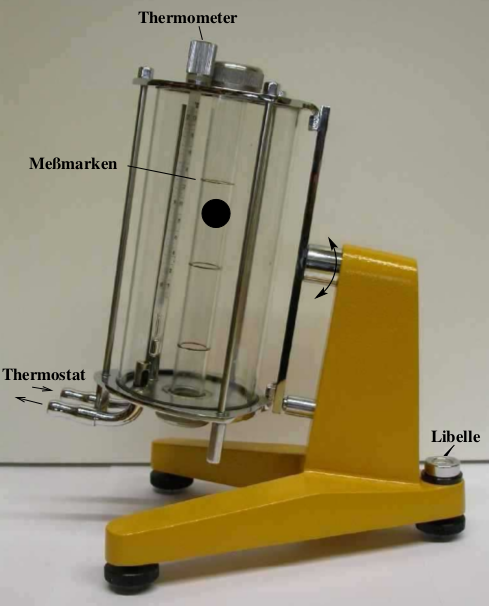
\includegraphics[width=0.6\textwidth]{viskosimeter.png}
  \caption{Aufbau des verwendeten Kugelfall-Viskosimeters \cite{sample}.}
\end{figure}
Vor Beginn der Messreihe wird der Durchmesser einer großen und einer kleinen
Glaskugel je zehn Mal gemessen und von beiden Kugeln wird die Masse bestimmt.
Ein Viskosimeter wie in Abbildung \ref{fig:viskosimeter.png} wird mit Hilfe der
Libelle gerade aufgestellt und das Rohr wird mit bidestilliertem Wasser gefüllt.
Dabei entstandene Luftblasen werden mit einem Glasstab aus dem Rohr gezogen.
Zuerst wird die kleinere der beiden Kugeln in das Rohr gelegt und das Rohr
verschlossen. Die Fallzeit, also die Zeit, die die Kugel von der obersten Messmarke
bis zur untersten Messmarkte braucht, wird zehn Mal gemessen. Dies wird für die
große Kugel wiederholt. Nach jeder Messung muss das Viskosimeter um $\SI{180}
{\celsius}$ gedreht werden.\newline
Zur Bestimmung der Temperaturabhänigkeit der Viskosität wird das Wasserbad, in
welchem sich das Fallrohr befindet, langsam bis $\SI{70}{\celsius}$ erhitzt
und für zehn Temperaturen je zweimal die Fallzeit bestimmt.
